\documentclass{beamer}

\usetheme{Madrid}
\usecolortheme{whale}
\usepackage{xcolor}
\usepackage{etoolbox}

\usepackage{graphicx}
\usepackage{hyperref}
\usepackage[backend=biber, sorting=none]{biblatex}
\addbibresource{refs.bib}
\DeclareFieldFormat*{title}{#1}
\DeclareFieldFormat*{url}{\newline\url{#1}\nopunct}
\DeclareFieldFormat{labelnumberwidth}{#1\adddot}
\setlength{\biblabelsep}{5pt}
\renewcommand*{\bibfont}{\tiny}
\usepackage{ragged2e}

\newcommand{\biburl}[2][]{%
  \newline - \ifstrempty{#1}{}{\textcolor{cyan}{#1: }}\url{#2}\nopunct
}


\title{ChatGPT Survey}
\subtitle{A Programmer's Perspective}
\author{Yu Zehan}
\institute{Intel FLEX}
\date{\today}

\begin{document}

\begin{frame}
  \titlepage
\end{frame}

\begin{frame}{Outline}
  \tableofcontents
\end{frame}

\section{Lifecycle of Coding}
\section{Prompt Engineering}
\section{Extensions and Plugins}
\section{Ecosystem}
\section{Websites}
\section{Limitations}

\begin{frame}{Lifecycle of Coding}
  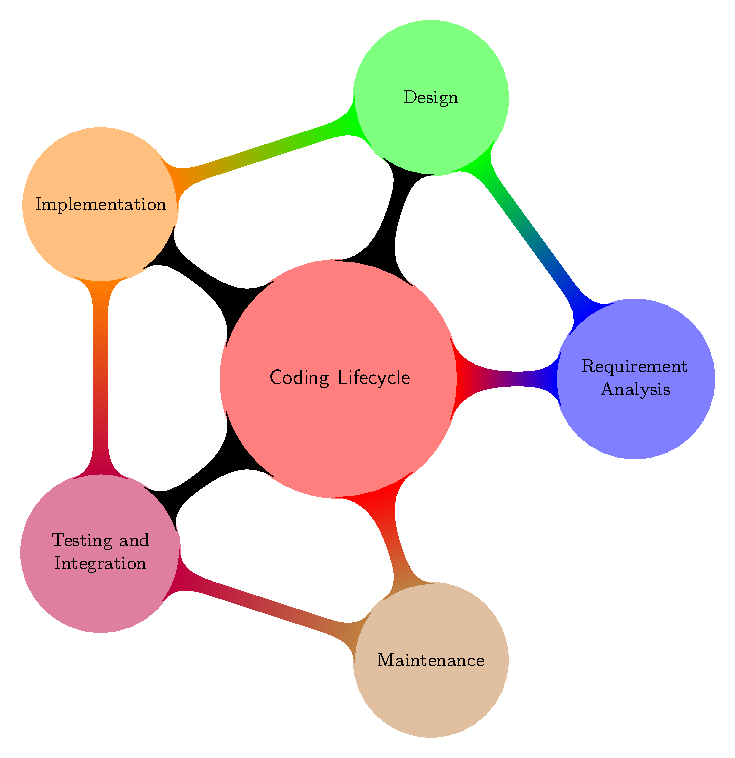
\includegraphics[width=\textwidth,height=0.8\textheight,keepaspectratio]{tikz-code-lifecycle.pdf}
\end{frame}



% 行动指南(instructions)、事实依据(facts)、思想纲领(policies)

\section{References}
\begin{frame}[t,allowframebreaks]{References}
  \nocite{*}
  \RaggedRight
  \printbibliography
\end{frame}


% Closing slide
\begin{frame}{FAQ}

\end{frame}

\end{document}
